%%  USB-TPLE
%%  Flyer für Embedded World 2010
%% 
%%  Andreas Müller, andz@gmx.de
%%  2010-02-26
%% 
\def\filename{flyer.tex}
\def\fileversion{v1.0}   % change this when leaflet-manual changed, too.
\def\filedate{2010/02/26}
\def\docdate {2010/02/26} % change this when leaflet-manual changed, too.
\listfiles
\errorcontextlines=99
\documentclass[
a4paper,
%%notumble,
%%nofoldmark,
%%dvipdfm,
%%portrait,
%%titlepage,
%%nocombine,
%%a3paper,
%%debug,
%%nospecialtricks,
%%draft,
]{leaflet}


\renewcommand*\foldmarkrule{.3mm}
\renewcommand*\foldmarklength{5mm}

\usepackage[T1]{fontenc}
\usepackage{textcomp}
\usepackage{mathptmx}
\usepackage[scaled=0.9]{helvet}
\makeatletter
\def\ptmTeX{T\kern-.1667em\lower.5ex\hbox{E}\kern-.075emX\@}
\DeclareRobustCommand{\ptmLaTeX}{L\kern-.3em
        {\setbox0\hbox{T}%
         %\vb@xt@ % :-)
         \vbox to\ht0{\hbox{%
                            \csname S@\f@size\endcsname
                            \fontsize\sf@size\z@
                            \math@fontsfalse\selectfont
                            A}%
                      \vss}%
        }%
        \kern-.12em
        \ptmTeX}
\makeatother
\let\TeX=\ptmTeX
\let\LaTeX=\ptmLaTeX
\usepackage{shortvrb}
\MakeShortVerb{\|}
\usepackage{url}
\usepackage{graphicx}
\usepackage[dvipsnames,usenames]{color}
\usepackage[ngerman]{babel}
\definecolor{LIGHTGRAY}{gray}{.9}
\definecolor{FHOrange}{rgb}{1.0,0.4,0.0}

%%%%\renewcommand{\descfont}{\normalfont}
\newcommand\Lpack[1]{\textsf{#1}}
\newcommand\Lclass[1]{\textsf{#1}}
\newcommand\Lopt[1]{\texttt{#1}}
\newcommand\Lprog[1]{\textit{#1}}

\newcommand*\defaultmarker{\textsuperscript\textasteriskcentered}

\newcommand{\changefont}[3]{ \fontfamily{#1} \fontseries{#2} \fontshape{#3} \selectfont}

\title{USB-TPLE}
\author{
  Andreas M\"uller, HS-Augsburg\\
  \\
  Prof. Dr. Hubert H\"ogl, HS-Augsburg}


%%\CutLine*{1}% Dotted line without scissors
\CutLine*{6}%  Dotted line without scissors

\AddToBackground{5}{%  Background of a small page
  \put(0,0){\textcolor{FHOrange}{\rule{\paperwidth}{\paperheight}}}}

\AddToBackground{6}{%  Background of a small page
  \put(0,0){\textcolor{FHOrange}{\rule{\paperwidth}{\paperheight}}}}

\AddToBackground*{2}{% Background of a large page
  \put(\LenToUnit{.5\paperwidth},\LenToUnit{0.15\paperheight}){%
    \makebox(0,0)[c]{%
      \resizebox{.9\paperwidth}{!}{{%
        \textsf{\textbf{\textcolor{LIGHTGRAY}{USB-TPLE}}}}}}}}

\begin{document}

%%\maketitle
%%\thispagestyle{empty}

%%\LARGE

%%\tableofcontents

\changefont{pag}{m}{n}


\begin{flushright}


\includegraphics [scale=0.2]{logo.png}

\end{flushright}

\begin{center}

\vskip 30pt

\Huge USB-TPLE\\

\bigskip

\vskip 30pt

\large Andreas M\"uller, HS-Augsburg\\Prof. Dr. Hubert H\"ogl, HS-Augsburg

\vskip 30pt

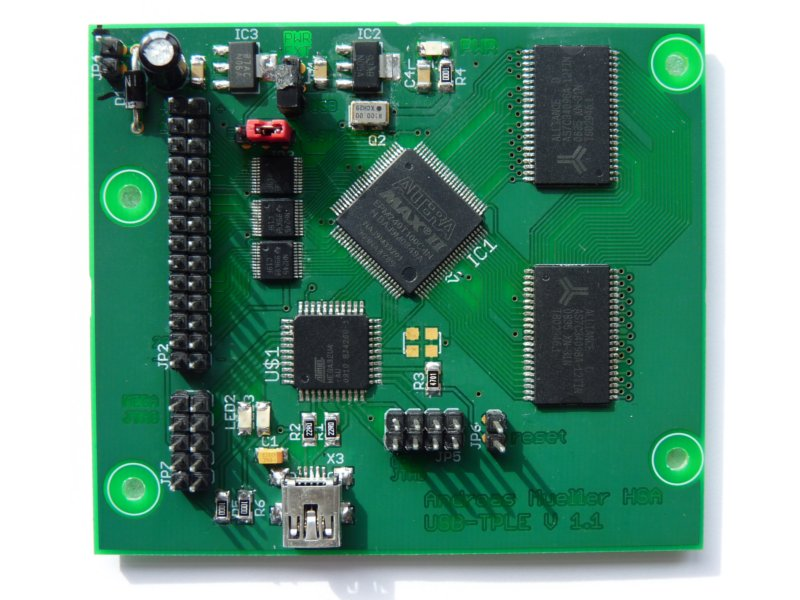
\includegraphics [scale=1.0]{board.jpg}

\vskip 30pt

\Large Ein universelles, rekonfigurierbares und freies USB Ger\"at, zur Timing-, Protokoll-, Logik- und Eventanalyse von digitalen Signalen
\end{center}

\eject

\section{\"Ubersicht}

USB-TPLE steht f"ur ein universelles, rekonfigurierbares und freies USB Ger\"at, zur Timing-, Protokoll-, Logik- und Eventanalyse von digitalen Signalen. Es wird derzeit im Zuge einer Bachelorarbeit von Andreas M"uller unter Leitung von Prof. Dr. Huber H"ogl an der Hochschule Augsburg enwickelt.

Hauptaufgabe des Projektes ist es, exakte Timing\-analysen an Mikrocontrollern oder "ahnlichem durchzuf"uhren. So kann zum Beispiel die Dauer eines Prozesses extern gemessen werden, ohne dass durch die Messung die Laufzeit beeinflusst wird.

Kerst"uck des Systems ist ein konfigurierbarer Logikbaustein (CPLD) der Firma Altera, sowie ein Mikrocontroller der Firma Atmel mit USB Anbindung. 

Das gesamte Projekt, sowohl Hard- als auch Software, ist im Sinne von Open-Source frei verf"ugbar und kann unter der URL

{\bf \underline \tt \large http://sta.informatik.fh-augsburg.de}

abgerufen werden. Auch ein SVN Repository mit TRAC ist unter dieser Adresse verf"ugbar.

\section{Funktionen}

Hauptfunktion ist, wie oben beschrieben, die Timinganalyse an Mikrocontrollern. Dazu wird zum Beispiel zu Beginn und zum Ende eines Prozesses ein Assemblerbefehl gesetzt, welcher einen Impuls auf einem IO Port des Mikrocontrollers ausgibt. Der Zeitpunkt des Impulses kann durch das Ger"at auf bis zu 0.1 Mikrosekunden genau aufgezeichnet werden.

Aufgrund der komplett freien Konfigurierbarkeit der Hardware sind jedoch auch weitere Anwendungen wie Protokoll- und Logikanalyse sowie auch ein Logikgenerator implementierbar.

\section{Hardware}

Beim Hardwaredesign wurde haupts"achlich darauf geachtet, dass nur Bauelemente verwendet wurden, welche frei verf"ugbar und erschwinglich sind. Im Vordergrund stand auch ein kompakter Aufbau und die m"oglichkeit der Stromversorgung sowohl "uber USB als auch "uber ein externes Netzteil. Beim aktuellen Prototypen sind auch alle Programmierschnittstellen der IC's nach aussen gef"uhrt. 

\subsection{Platinendesign}

Das Platinendesign ist wie das gesamte Projekt als Open Source verf"ugbar. Alle Schaltpl"ane und PCB-Designs wurden mit der Software EAGLE von Cadsoft erstellt.\\
Nachfolgend sind alle Eigenschaften des Platinendesigns aufgelistet.

\begin{itemize}
  \item Gr"o"stenteils SMD Bauweise
  \item 2 Schichtiges Layout
  \item Stromversorgung "uber Jumper einstellbar (USB/ext.)
  \item Messpannung w"ahlbar (3.3V/5.0V)
\end{itemize}

\subsection{Prozessor}

Als CPU kommt ein Mikrocontroller der Firma Atmel zum Einsatz. Der ATMEGA32U4 ist ein Controller der 8-bit AVR Serie mit den folgenden Eigenschaften.

\begin{itemize}
  \item 32KB Flashspeicher
  \item 2.5KB RAM
  \item Integrierte USB Schnittstelle
  \item Bootloader (Konfigurierbar u"ber USB)
\end{itemize}

Die Software f"ur den Mikrocontroller ist haupts"achlich in C geschrieben. Er ist "uber einen 4-bit breiten, synchronen Datenbus mit dem Logikbaustein verbunden.

\subsection{CPLD}

Als Logikbaustein wird ein Low-Cost CPLD der Firma Altera verwendet. Der CPLD der MAX II Serie ist mit 100MHz getaktet und "uber einen 16-bit breiten Datenbus mit einem externen, schnellen RAM verbunden. Als Hardwarebeschreibungssprache kommt VHDL zum Einsatz und als Synthesetool wird das kostenlose Quartus II der Herstellerfirma verwendet.

\begin{itemize}
  \item 240 Logikzellen
  \item Konfigurierbar "uber JTAG oder direkt durch den Mikrocontroller
  \item 8K integrierter UFM
  \item 24 IO Ports f"ur Messungen verf"ugbar
\end{itemize}

\subsection{Sonstiges}

Weitere verwendete Bauelemente sind zum Beispiel die Bustreiber, welche es erm"oglichen sowohl 3.3V als auch 5V Bausteine zu analysieren. Auch dienen die Bustreiber als Schutz des CPLD.

Als Speicher kommen zwei 256K*16 Bausteine zum Einsatz. Dadurch k"onnen bis zu 512.000 Events aufgezeichnet und weiterverarbeitet werden. 

\section{Software}

Gesteuert werden kann das System mit jedem beliebigen Terminalprogramm "uber einen virtuellen COM Port. Dazu werden AT-"ahnliche Befehle an den Mikrocontroller geschickt.

Als Speicherformat wird das Value-Change-Dump Format verwendet. Dieses ASCII basierende Format f"ur Logiksignale hat den Vorteil, dass es zum einen problemlos "uber ein Terminal genutzt werden kann, zum anderen kann das Open-Source Programm GTK-WAVE mit diesem Dateiformat umgehen.

Geplant ist auch ein grafisches Frontend f"ur die komfortable Steuerung des USB-TPLE sowohl unter Linux als auch unter Windows. Um die Plattformunabh"angikeit zu erreichen, wird diese Software mit der QT Bibliothek von Nokia erstellt werden.

\section{Entwicklungsstatus}

Das gesamte Projekt befindet sich derzeit noch in einem sehr fr"uhen Entwicklungsstatus.

Bis jetzt fertigestellt ist der Hardwarentwurf sowie die Produktion des ersten Prototypen. Die Enwicklung der CPLD- und Mikrocontroller-Firmware befindet sich noch in der Entwurfsphase und ist daher noch nicht Funktionsf"ahig.

Der aktuelle Status kann auf der Projektseite eingesehen werden:

\vskip 30pt

\begin{center}
{\Large \tt sta.informatik.fh-augsburg.de}
\end{center}

\eject

\vspace*{\fill}

USB-TPLE\\Andreas M"uller\\Hochschule Augsburg\\sta.informatik.fh-augsburg.de\\andreas.mueller@hs-augsburg.de

%%\endgroup
\end{document}

%%
%% End of file `leaflet-manual.tex'.
